% INTRODUCTION CHAPTER
\chapter{Introduction}\label{ch:introduction}

\section{Context}\label{sec:Context}

Esports is a form of competition using video games where participants will compete either individually or in a team for a chance at victory.
These competitions attract millions of viewers, with estimates of 532 million spectators by the end of 2022, and this value is expected to grow annually at a value of roughly 8.7\%~\citep{newzoo2022viewers}.
The rapid growth in Esports has led to the industry becoming professional, with hundreds of players contracted on full-time contracts competing for prize pools of up to \$40 million~\citep{esportsearnings}.
According to~\citet{newzoo2022viewers} this viewership will help the industry generate over \$1.38 billion in revenue by the end of 2022.
As the Esports industry continues to grow, so does the importance on teams to win and remain relevant in the industry.\\

In traditional sports, analytics have become an extremely popular field with teams investing heavily in some form of analytics.
These analytics can be used from evaluating opposing teams, to individual player forecasting and even used to decide signings or team selection~\citep{sarlis2020sports, apostolou2019sports}.
\citet{apostolou2019sports, sarlis2020sports} shows that these analytics can be applied for each athlete, giving an accurate estimation of key metrics such as goals scored per season or the number of shots attempted in a given match.
This same methodology could be applied to Esports, using these machine learning techniques could highlight specific factors in-game helping analysts and coaches refine strategies within the game.\\

The ease of data collection coming from each match has to led to a massive rise in Esports analytics.
In-depth analysis of matches, teams and in-game factors become key techniques for teams to gain this advantage over their competitors, with teams being required by their leagues to have at least one dedicated coach and analyst similar to traditional sports teams~\citep{LCSRules}.
These coaches and analysts use predictive analytics to maximise their team's likelihood of winning by altering numerous features related to in-game strategies, current `meta-game' analysis and common patterns of their competition~\citep{kokkinakis2021metagaming}.
However, this analysis is often completed manually by watching key highlights of matches using the analyst's intuition and using rudimentary analysis of in-game factors.\\

If matches can be accurately predicted using machine learning techniques, then analysts can provide new opportunities to optimise player strategies and can lead their teams to better outcomes.
Applying the same findings found in~\citet{gray2012customer}, it can be seen that the overall performance and fan satisfaction with a sports team's performance has a measurable impact on revenue via fan attendance and their media response.
Esports fans also appear to increasingly demand skillful performances especially from players that are deemed as \emph{'superstars'}, with these players being more likely to attract new viewers, thus increasing the economic gain of the market~\citep{mangeloja2019economics, ward2019esport}.
It would then be in the interest of both teams and individual players to maximise their abilities and career longevity using these advanced analytics, so they can fully realise their potential;
especially when the volatility of a players job security results in only the top 10\% of players having stable careers~\citep{ward2019esport}.\\


\section{League of Legends}\label{sec:League of Legends}

A \ac{MOBA} is fusion genre of real-time strategy, role-playing and action games in which two sets of teams will compete in a known arena.
The objective of each game is to defeat the opposition by destroying the enemy's base.
Each player will select and control a unique~\gls{champion} with their own set of distinct abilities, this~\gls{champion} will be selected before the game starts and cannot be changed until the game has ended.
Players can strengthen their~\glspl{champion} by gaining experience and gold, this can be done by slaying enemy~\glspl{minion}, \gls{jungle} monsters, enemy structures or enemy \glspl{champion}.
This gold can be spent in the shop allowing players to purchase items that enhance the attributes of their \gls{champion}, as well as various utility items such as \glspl{ward}.

League of Legends is a \ac{MOBA} game developed by Riot Games released in 2009, it is one of most popular esports games in the world with over 180 million monthly players and a peak of 73.8 million concurrent viewers~\citep{riotplayercount, upcomerworld2021}.
The map of League of Legends can be seen in Figure~\ref{fig:Lolmap}.

\begin{figure}[h]
    \centering
    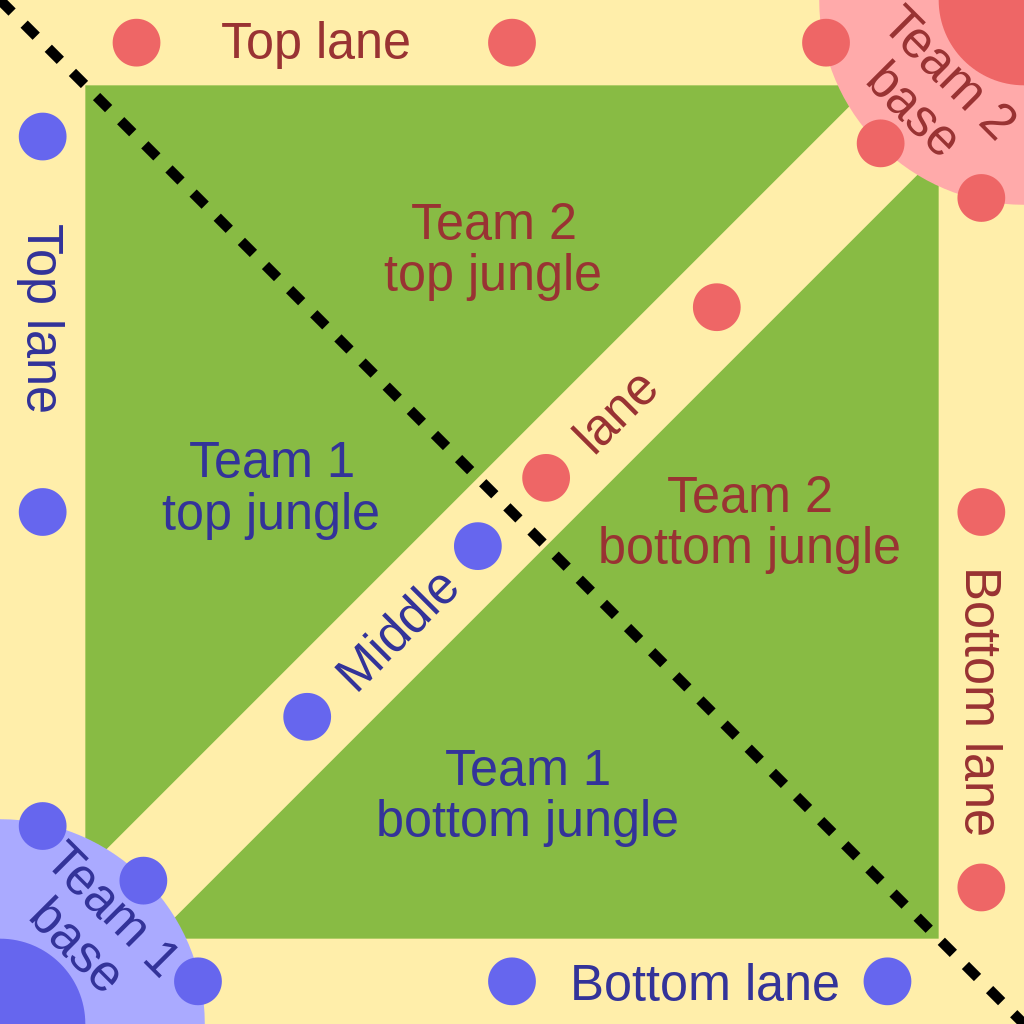
\includegraphics[width=0.75\textwidth]{figures/MOBAMap}
    \caption{Map of League of Legends}
    \label{fig:Lolmap}
\end{figure}


\gls{buff} \gls{nerf}  \gls{baron} \gls{dragon} \gls{rift herald} \gls{nexus} \gls{tower} \gls{meta} \gls{inhibitor}



\section{Structure}\label{sec:Structure}
\lipsum[1-5]

\section{Aims and Objectives}\label{sec:Aims and Objectives}

Objective: \begin{quote}  \emph{Can the outcome of a League of Legends match be predicted using in-game factors?} \end{quote}